
%% bare_conf.tex
%% V1.3
%% 2007/01/11
%% by Michael Shell
%% See:
%% http://www.michaelshell.org/
%% for current contact information.
%%
%% This is a skeleton file demonstrating the use of IEEEtran.cls
%% (requires IEEEtran.cls version 1.7 or later) with an IEEE conference paper.
%%
%% Support sites:
%% http://www.michaelshell.org/tex/ieeetran/
%% http://www.ctan.org/tex-archive/macros/latex/contrib/IEEEtran/
%% and
%% http://www.ieee.org/

%%*************************************************************************
%% Legal Notice:
%% This code is offered as-is without any warranty either expressed or
%% implied; without even the implied warranty of MERCHANTABILITY or
%% FITNESS FOR A PARTICULAR PURPOSE! 
%% User assumes all risk.
%% In no event shall IEEE or any contributor to this code be liable for
%% any damages or losses, including, but not limited to, incidental,
%% consequential, or any other damages, resulting from the use or misuse
%% of any information contained here.
%%
%% All comments are the opinions of their respective authors and are not
%% necessarily endorsed by the IEEE.
%%
%% This work is distributed under the LaTeX Project Public License (LPPL)
%% ( http://www.latex-project.org/ ) version 1.3, and may be freely used,
%% distributed and modified. A copy of the LPPL, version 1.3, is included
%% in the base LaTeX documentation of all distributions of LaTeX released
%% 2003/12/01 or later.
%% Retain all contribution notices and credits.
%% ** Modified files should be clearly indicated as such, including  **
%% ** renaming them and changing author support contact information. **
%%
%% File list of work: IEEEtran.cls, IEEEtran_HOWTO.pdf, bare_adv.tex,
%%                    bare_conf.tex, bare_jrnl.tex, bare_jrnl_compsoc.tex
%%*************************************************************************

% *** Authors should verify (and, if needed, correct) their LaTeX system  ***
% *** with the testflow diagnostic prior to trusting their LaTeX platform ***
% *** with production work. IEEE's font choices can trigger bugs that do  ***
% *** not appear when using other class files.                            ***
% The testflow support page is at:
% http://www.michaelshell.org/tex/testflow/



% Note that the a4paper option is mainly intended so that authors in
% countries using A4 can easily print to A4 and see how their papers will
% look in print - the typesetting of the document will not typically be
% affected with changes in paper size (but the bottom and side margins will).
% Use the testflow package mentioned above to verify correct handling of
% both paper sizes by the user's LaTeX system.
%
% Also note that the "draftcls" or "draftclsnofoot", not "draft", option
% should be used if it is desired that the figures are to be displayed in
% draft mode.
%
\documentclass[conference]{IEEEtran}
% Add the compsoc option for Computer Society conferences.
%
% If IEEEtran.cls has not been installed into the LaTeX system files,
% manually specify the path to it like:
% \documentclass[conference]{../sty/IEEEtran}





% Some very useful LaTeX packages include:
% (uncomment the ones you want to load)


% *** MISC UTILITY PACKAGES ***
%
%\usepackage{ifpdf}
% Heiko Oberdiek's ifpdf.sty is very useful if you need conditional
% compilation based on whether the output is pdf or dvi.
% usage:
% \ifpdf
%   % pdf code
% \else
%   % dvi code
% \fi
% The latest version of ifpdf.sty can be obtained from:
% http://www.ctan.org/tex-archive/macros/latex/contrib/oberdiek/
% Also, note that IEEEtran.cls V1.7 and later provides a builtin
% \ifCLASSINFOpdf conditional that works the same way.
% When switching from latex to pdflatex and vice-versa, the compiler may
% have to be run twice to clear warning/error messages.






% *** CITATION PACKAGES ***
%
\usepackage{cite}
% cite.sty was written by Donald Arseneau
% V1.6 and later of IEEEtran pre-defines the format of the cite.sty package
% \cite{} output to follow that of IEEE. Loading the cite package will
% result in citation numbers being automatically sorted and properly
% "compressed/ranged". e.g., [1], [9], [2], [7], [5], [6] without using
% cite.sty will become [1], [2], [5]--[7], [9] using cite.sty. cite.sty's
% \cite will automatically add leading space, if needed. Use cite.sty's
% noadjust option (cite.sty V3.8 and later) if you want to turn this off.
% cite.sty is already installed on most LaTeX systems. Be sure and use
% version 4.0 (2003-05-27) and later if using hyperref.sty. cite.sty does
% not currently provide for hyperlinked citations.
% The latest version can be obtained at:
% http://www.ctan.org/tex-archive/macros/latex/contrib/cite/
% The documentation is contained in the cite.sty file itself.






% *** GRAPHICS RELATED PACKAGES ***
%
\ifCLASSINFOpdf
  \usepackage[pdftex]{graphicx}
  % declare the path(s) where your graphic files are
  % \graphicspath{{../pdf/}{../jpeg/}}
  \graphicspath{./figures/}
  % and their extensions so you won't have to specify these with
  % every instance of \includegraphics
  \DeclareGraphicsExtensions{.pdf,.jpeg,.png}
\else
  % or other class option (dvipsone, dvipdf, if not using dvips). graphicx
  % will default to the driver specified in the system graphics.cfg if no
  % driver is specified.
  % \usepackage[dvips]{graphicx}
  % declare the path(s) where your graphic files are
  % \graphicspath{{../eps/}}
  % and their extensions so you won't have to specify these with
  % every instance of \includegraphics
  % \DeclareGraphicsExtensions{.eps}
\fi
% graphicx was written by David Carlisle and Sebastian Rahtz. It is
% required if you want graphics, photos, etc. graphicx.sty is already
% installed on most LaTeX systems. The latest version and documentation can
% be obtained at: 
% http://www.ctan.org/tex-archive/macros/latex/required/graphics/
% Another good source of documentation is "Using Imported Graphics in
% LaTeX2e" by Keith Reckdahl which can be found as epslatex.ps or
% epslatex.pdf at: http://www.ctan.org/tex-archive/info/
%
% latex, and pdflatex in dvi mode, support graphics in encapsulated
% postscript (.eps) format. pdflatex in pdf mode supports graphics
% in .pdf, .jpeg, .png and .mps (metapost) formats. Users should ensure
% that all non-photo figures use a vector format (.eps, .pdf, .mps) and
% not a bitmapped formats (.jpeg, .png). IEEE frowns on bitmapped formats
% which can result in "jaggedy"/blurry rendering of lines and letters as
% well as large increases in file sizes.
%
% You can find documentation about the pdfTeX application at:
% http://www.tug.org/applications/pdftex





% *** MATH PACKAGES ***
%
%\usepackage[cmex10]{amsmath}
% A popular package from the American Mathematical Society that provides
% many useful and powerful commands for dealing with mathematics. If using
% it, be sure to load this package with the cmex10 option to ensure that
% only type 1 fonts will utilized at all point sizes. Without this option,
% it is possible that some math symbols, particularly those within
% footnotes, will be rendered in bitmap form which will result in a
% document that can not be IEEE Xplore compliant!
%
% Also, note that the amsmath package sets \interdisplaylinepenalty to 10000
% thus preventing page breaks from occurring within multiline equations. Use:
%\interdisplaylinepenalty=2500
% after loading amsmath to restore such page breaks as IEEEtran.cls normally
% does. amsmath.sty is already installed on most LaTeX systems. The latest
% version and documentation can be obtained at:
% http://www.ctan.org/tex-archive/macros/latex/required/amslatex/math/





% *** SPECIALIZED LIST PACKAGES ***
%
%\usepackage{algorithmic}
% algorithmic.sty was written by Peter Williams and Rogerio Brito.
% This package provides an algorithmic environment fo describing algorithms.
% You can use the algorithmic environment in-text or within a figure
% environment to provide for a floating algorithm. Do NOT use the algorithm
% floating environment provided by algorithm.sty (by the same authors) or
% algorithm2e.sty (by Christophe Fiorio) as IEEE does not use dedicated
% algorithm float types and packages that provide these will not provide
% correct IEEE style captions. The latest version and documentation of
% algorithmic.sty can be obtained at:
% http://www.ctan.org/tex-archive/macros/latex/contrib/algorithms/
% There is also a support site at:
% http://algorithms.berlios.de/index.html
% Also of interest may be the (relatively newer and more customizable)
% algorithmicx.sty package by Szasz Janos:
% http://www.ctan.org/tex-archive/macros/latex/contrib/algorithmicx/




% *** ALIGNMENT PACKAGES ***
%
%\usepackage{array}
% Frank Mittelbach's and David Carlisle's array.sty patches and improves
% the standard LaTeX2e array and tabular environments to provide better
% appearance and additional user controls. As the default LaTeX2e table
% generation code is lacking to the point of almost being broken with
% respect to the quality of the end results, all users are strongly
% advised to use an enhanced (at the very least that provided by array.sty)
% set of table tools. array.sty is already installed on most systems. The
% latest version and documentation can be obtained at:
% http://www.ctan.org/tex-archive/macros/latex/required/tools/


%\usepackage{mdwmath}
%\usepackage{mdwtab}
% Also highly recommended is Mark Wooding's extremely powerful MDW tools,
% especially mdwmath.sty and mdwtab.sty which are used to format equations
% and tables, respectively. The MDWtools set is already installed on most
% LaTeX systems. The lastest version and documentation is available at:
% http://www.ctan.org/tex-archive/macros/latex/contrib/mdwtools/


% IEEEtran contains the IEEEeqnarray family of commands that can be used to
% generate multiline equations as well as matrices, tables, etc., of high
% quality.


%\usepackage{eqparbox}
% Also of notable interest is Scott Pakin's eqparbox package for creating
% (automatically sized) equal width boxes - aka "natural width parboxes".
% Available at:
% http://www.ctan.org/tex-archive/macros/latex/contrib/eqparbox/





% *** SUBFIGURE PACKAGES ***
%\usepackage[tight,footnotesize]{subfigure}
% subfigure.sty was written by Steven Douglas Cochran. This package makes it
% easy to put subfigures in your figures. e.g., "Figure 1a and 1b". For IEEE
% work, it is a good idea to load it with the tight package option to reduce
% the amount of white space around the subfigures. subfigure.sty is already
% installed on most LaTeX systems. The latest version and documentation can
% be obtained at:
% http://www.ctan.org/tex-archive/obsolete/macros/latex/contrib/subfigure/
% subfigure.sty has been superceeded by subfig.sty.



%\usepackage[caption=false]{caption}
%\usepackage[font=footnotesize]{subfig}
% subfig.sty, also written by Steven Douglas Cochran, is the modern
% replacement for subfigure.sty. However, subfig.sty requires and
% automatically loads Axel Sommerfeldt's caption.sty which will override
% IEEEtran.cls handling of captions and this will result in nonIEEE style
% figure/table captions. To prevent this problem, be sure and preload
% caption.sty with its "caption=false" package option. This is will preserve
% IEEEtran.cls handing of captions. Version 1.3 (2005/06/28) and later 
% (recommended due to many improvements over 1.2) of subfig.sty supports
% the caption=false option directly:
%\usepackage[caption=false,font=footnotesize]{subfig}
%
% The latest version and documentation can be obtained at:
% http://www.ctan.org/tex-archive/macros/latex/contrib/subfig/
% The latest version and documentation of caption.sty can be obtained at:
% http://www.ctan.org/tex-archive/macros/latex/contrib/caption/




% *** FLOAT PACKAGES ***
%
%\usepackage{fixltx2e}
% fixltx2e, the successor to the earlier fix2col.sty, was written by
% Frank Mittelbach and David Carlisle. This package corrects a few problems
% in the LaTeX2e kernel, the most notable of which is that in current
% LaTeX2e releases, the ordering of single and double column floats is not
% guaranteed to be preserved. Thus, an unpatched LaTeX2e can allow a
% single column figure to be placed prior to an earlier double column
% figure. The latest version and documentation can be found at:
% http://www.ctan.org/tex-archive/macros/latex/base/



%\usepackage{stfloats}
% stfloats.sty was written by Sigitas Tolusis. This package gives LaTeX2e
% the ability to do double column floats at the bottom of the page as well
% as the top. (e.g., "\begin{figure*}[!b]" is not normally possible in
% LaTeX2e). It also provides a command:
%\fnbelowfloat
% to enable the placement of footnotes below bottom floats (the standard
% LaTeX2e kernel puts them above bottom floats). This is an invasive package
% which rewrites many portions of the LaTeX2e float routines. It may not work
% with other packages that modify the LaTeX2e float routines. The latest
% version and documentation can be obtained at:
% http://www.ctan.org/tex-archive/macros/latex/contrib/sttools/
% Documentation is contained in the stfloats.sty comments as well as in the
% presfull.pdf file. Do not use the stfloats baselinefloat ability as IEEE
% does not allow \baselineskip to stretch. Authors submitting work to the
% IEEE should note that IEEE rarely uses double column equations and
% that authors should try to avoid such use. Do not be tempted to use the
% cuted.sty or midfloat.sty packages (also by Sigitas Tolusis) as IEEE does
% not format its papers in such ways.





% *** PDF, URL AND HYPERLINK PACKAGES ***
%
%\usepackage{url}
% url.sty was written by Donald Arseneau. It provides better support for
% handling and breaking URLs. url.sty is already installed on most LaTeX
% systems. The latest version can be obtained at:
% http://www.ctan.org/tex-archive/macros/latex/contrib/misc/
% Read the url.sty source comments for usage information. Basically,
% \url{my_url_here}.





% *** Do not adjust lengths that control margins, column widths, etc. ***
% *** Do not use packages that alter fonts (such as pslatex).         ***
% There should be no need to do such things with IEEEtran.cls V1.6 and later.
% (Unless specifically asked to do so by the journal or conference you plan
% to submit to, of course. )


% correct bad hyphenation here
\hyphenation{op-tical net-works semi-conduc-tor UbiApp UbiComp}


\begin{document}
%
% paper title
% can use linebreaks \\ within to get better formatting as desired
% \title{Interacting with the environment: a framework to develop ubiquitous applications for intelligent environments}
\title{Encapsulating the environment: a flexible framework to develop ubiquitous applications for intelligent environments}


% author names and affiliations
% use a multiple column layout for up to three different
% affiliations
\author{\IEEEauthorblockN{Matheus Erthal}
\IEEEauthorblockA{Institute of Computing\\
Federal Fluminense University\\
Rio de Janeiro, Brazil\\
Email: merthal@ic.uff.br}
\and
\IEEEauthorblockN{David Barreto}
\IEEEauthorblockA{Institute of Computing\\
Federal Fluminense University\\
Email: dbarreto@ic.uff.br}
\and
\IEEEauthorblockN{Douglas Mareli}
\IEEEauthorblockA{Institute of Computing\\
Federal Fluminense University\\
Email: dmareli@ic.uff.br}
\and
\IEEEauthorblockN{Orlando Loques}
\IEEEauthorblockA{Institute of Computing\\
Federal Fluminense University\\
Email: loques@ic.uff.br}}
% \author{\IEEEauthorblockN{Michael Shell}
% \IEEEauthorblockA{School of Electrical and\\Computer Engineering\\
% Georgia Institute of Technology\\
% Atlanta, Georgia 30332--0250\\
% Email: http://www.michaelshell.org/contact.html}
% \and
% \IEEEauthorblockN{Homer Simpson}
% \IEEEauthorblockA{Twentieth Century Fox\\
% Springfield, USA\\
% Email: homer@thesimpsons.com}
% \and
% \IEEEauthorblockN{James Kirk\\ and Montgomery Scott}
% \IEEEauthorblockA{Starfleet Academy\\
% San Francisco, California 96678-2391\\
% Telephone: (800) 555--1212\\
% Fax: (888) 555--1212}}

% conference papers do not typically use \thanks and this command
% is locked out in conference mode. If really needed, such as for
% the acknowledgment of grants, issue a \IEEEoverridecommandlockouts
% after \documentclass

% for over three affiliations, or if they all won't fit within the width
% of the page, use this alternative format:
% 
%\author{\IEEEauthorblockN{Michael Shell\IEEEauthorrefmark{1},
%Homer Simpson\IEEEauthorrefmark{2},
%James Kirk\IEEEauthorrefmark{3}, 
%Montgomery Scott\IEEEauthorrefmark{3} and
%Eldon Tyrell\IEEEauthorrefmark{4}}
%\IEEEauthorblockA{\IEEEauthorrefmark{1}School of Electrical and Computer Engineering\\
%Georgia Institute of Technology,
%Atlanta, Georgia 30332--0250\\ Email: see http://www.michaelshell.org/contact.html}
%\IEEEauthorblockA{\IEEEauthorrefmark{2}Twentieth Century Fox, Springfield, USA\\
%Email: homer@thesimpsons.com}
%\IEEEauthorblockA{\IEEEauthorrefmark{3}Starfleet Academy, San Francisco, California 96678-2391\\
%Telephone: (800) 555--1212, Fax: (888) 555--1212}
%\IEEEauthorblockA{\IEEEauthorrefmark{4}Tyrell Inc., 123 Replicant Street, Los Angeles, California 90210--4321}}




% use for special paper notices
%\IEEEspecialpapernotice{(Invited Paper)}




% make the title area
\maketitle


\begin{abstract}
%\boldmath
Due to recent advances in mobile computing and wireless communication technologies, we can see the emergence of a favourable scenario for building ubiquitous/pervasive applications. This work proposes a new framework that aims at building those applications, providing a set of concepts and implementation tools. We propose abstractions that allow developers to handle the resources spread in the environment in a simple and homogeneous way, and to interpret context information. In order to demonstrate the feasibility of the proposal, the concepts were implemented in a platform named \textit{SmartAndroid}. A ubiquitous applications prototyping interface was implemented over this platform to allow testing of different environment configurations before purchasing all devices; and also a context rules composition interface, where end users can define their preferences in the environment.

% Context awareness is reaching increasingly visibility in the current applications development scenario. The goal of this paper is to propose a new solution for representing, distributing and interpreting context informations, thus allowing the construction of applications for intelligent ambients. The infrastructure described in this paper exposes the ambient resources in a higher level, leading to a simpler and more dynamic creation of context rules; and by means of a graphical interface, end users are able to easily create and customize rules in the ambient. The proposed concepts have been implemented as a platform focused on building smart homes.
% 
% This article describes the Pervasive Applications Prototyping and Management Interface (IPGAP) that aims to provide a platform to support construction, test and execution of applications for smart ambients. In order to provide these features capabilities, our tool helps to perform simulation of sensors and actuators as well as means to visualize the interaction of real components which are inside the ambient. This way the developer will be able to construct applications without having a complete smart ambient infrastructure.

\end{abstract}
% IEEEtran.cls defaults to using nonbold math in the Abstract.
% This preserves the distinction between vectors and scalars. However,
% if the conference you are submitting to favors bold math in the abstract,
% then you can use LaTeX's standard command \boldmath at the very start
% of the abstract to achieve this. Many IEEE journals/conferences frown on
% math in the abstract anyway.

% no keywords




% For peer review papers, you can put extra information on the cover
% page as needed:
% \ifCLASSOPTIONpeerreview
% \begin{center} \bfseries EDICS Category: 3-BBND \end{center}
% \fi
%
% For peerreview papers, this IEEEtran command inserts a page break and
% creates the second title. It will be ignored for other modes.
\IEEEpeerreviewmaketitle



% %%%%%%%%%%%%%%%%%%%%%%%%%%%%%%%%%%%%
%              SECTION
% %%%%%%%%%%%%%%%%%%%%%%%%%%%%%%%%%%%%
\section{Introduction}
% no \IEEEPARstart
% You must have at least 2 lines in the paragraph with the drop letter
% (should never be an issue)
The field of Ubiquitous Computing (UbiComp), nowadays widely discussed, was first proposed by Mark Weiser in the 1990's~\cite{Weiser1991century}. Also referred by pervasive computing, the field aims at providing a different paradigm of human-machine interaction. As traditional applications provides services to users through their explicit interaction (using devices as mouse, keyword, monitor, for example), in ubiquitous applications (UbiApp) the interaction happens without the need of explicit interaction, i.e. the application tries to discover the users needs through the acquisition of context (using sensors) and the knowledge of their preferences, and providing services in the environment (using actuators). These environments enhanced with sensors and actuators to provide automated services to persons are also called Intelligent Environments (IE).

% The construction of a UbiApp from the start is not a simple task, since the developer will have concerns from the communication level to the representation of resources in high level before even start programming the business logic of her application. 
The construction and manipulation of UbiApps represent major challenges for developers, especially in terms of technical knowledge required and the availability of real devices during application development. Some of these challenges can be well highlighted: (i) there are difficulties in establishing a common protocol for communication between the components of the distributed system, because of the \textit{heterogeneity of devices} involved, (ii) the interactivity of UbiApps is hampered depending on the amount and \textit{variety of context information and services} available in the environment, (iii) \textit{developing and testing applications} require high availability of resources, such as sensors (e.g. presence, lighting, temperature), actuators (e.g. keys, alarms, smart-tvs), including new embedded devices, or physical spaces, such as a house for applications of type smart home.

% From the Mark Weiser proposed in the 1990s, researchers in the field of ubicomp / pervasive have proposed changes in human-machine interaction, in order to make the use of devices increasingly transparent environment. This enables the user to focus on the task at hand and not the tool to do it. From these ideas came the concept of smart environments, where sensors and actuators interconnected network are able to provide relevant information about the environment to applications and users, and effectively act in this environment and change its state.



%FIXME: araujo � um artigo em PT, arrumar um em EN
In this work we propose a framework for developing UbiApps in IE. The goal is to provide support for the programming, testing and execution of applications, thus allowing to deal consistently with systems great complexity. The framework stands out for addressing the challenges already identified in UbiComp~\cite{araujo2003}. The \textit{heterogeneity of devices} is handled through the definition of a Distributed Component Model, that provides abstractions to encapsulate these devices, also called resources, enabling developers to interact with them seamlessly. Regarding the \textit{variety of context information and services} issue, we propose a solution for context interpretation that allows developers to create and manage context rules at runtime, and users to set their preferences in the IE. Finally, regarding the issue on the \textit{resource availability}, the framework includes an application interface for the prototyping and management of pervasive applications (IPGAP), focused on visualization and testing UbiApps, mixing real and virtual components.
%in which the basic component has a uniform structure defined as a Resource Agent (RA), formerly proposed in~\cite{cardoso2006} as an entity gathering context information. In this work, the RA, while maintaining context information, acts as a component that encapsulates the device code associated with it, including aspects of interaction with application components. 
%The \textit{heterogeneity of devices} is handled through the definition of a Distributed Component Model, in which the basic component has a uniform structure defined as a Resource Agent (RA), formerly proposed in~\cite{cardoso2006} as an entity gathering context information. In this work, the RA, while maintaining context information, acts as a component that encapsulates the device code associated with it, including aspects of interaction with application components. 

The concepts of the framework were materialized on a platform called \textit{SmartAndroid}\footnote{www.tempo.uff.br/smartandroid}, whose development has enabled appraisal in order to prove that the conceptual framework facilitates the process of building UbiApps. We implemented some use cases to validate different aspects of the framework proposed and to testify its capabilities, supported by the elaboration of competency questions, which is a mechanism mostly used to evaluate ontologies, but can also be used as an assessment to this work. 
%power of representation 
%testify the feasibility 
% has enabled the construction of use cases that demonstrate the effectiveness of the approach to provide context awareness to new applications.

% The concepts of the framework have been implemented on a platform called \textit{SmartAndroid}\footnote{www.tempo.uff.br/smartandroid} developed in the context of the project. The implementation of this project has enabled appraisal in order to prove that the conceptual framework facilitates the process of building UbiApps.  One of the evaluations occurred during the processing of an application running on a purely local UbiApp. In another assessment, an application was built to verify the feasibility of implementation of Context Model, through the exploitation of communication mechanisms used in the Distributed Component Model.


The remainder of this paper is organized as follows. First we present in Section~\ref{sec:overview} an overview of the main concepts used as a basis for the framework's development. In Section~\ref{sec:framework}, we present the framework's overall architecture and main features. We then, in Section~\ref{sec:evaluation}, present a proof of concept demonstrating the feasibility of building UbiApps using the framework and we show examples of applications that explores the key features of the IE. Finally, in Section~\ref{sec:related} we compare our approach with related work and in Section~\ref{sec:conclusion} we conclude this paper with the main remarks.
[refactor this paragraph]


% %%%%%%%%%%%%%%%%%%%%%%%%%%%%%%%%%%%%
%              SECTION
% %%%%%%%%%%%%%%%%%%%%%%%%%%%%%%%%%%%%
\section{Related Work} \label{sec:related}
% [ubicomp is nice but it is not priceless]
The benefits to users and developers that UbiComp foresees reach beyond the horizon of many imaginative researchers. The possibilities that arise from it surpass the bounds established by keyboards and mice, our standard interfaces. Nonetheless, building such adaptable applications requires much effort from developers that see themselves immersed in a universe of device's specifications and communication technologies, apart from the problem itself that the application must solve. Therefore, many researchers have focused on diminishing those obstacles by providing abstractions, middlewares, services, tools, and other supportive techniques, not only for development but also for prototyping.

%ubicomp implies dealing with limited and dynamically varying computational resources [kindberg2002ieee]

Most approaches focus on one aspect of UbiComp, such as security~\cite{}, location~\cite{}, context representation~\cite{}, SmartHome specific~\cite{dixon2012operating}, among others. [+++]
% The works that focus on context interpretation/context rules
% Some works focus on composing and managing context rules  %About the adaptability 
%Challenges in Access Right Assignment for Secure Home Networks - 17



%TODO: Gaia
As one of the most famous, the Gaia middleware is designed to facilitate the construction of applications for IE. It consists of a set of core services and a framework for building distributed context aware applications. The Gaia embraces many goals that include the acquisition of context, the maintenance of hardware and software descriptions, mechanisms to find resources and to compose context rules, among others.
%uses operating systems abstractions to define its architecture
%have many goals that include the provision of mechanisms of acquisition of context; composition of rules (using first logic order), 
%%maintenance of hardwares and softwares description and about applications; 
%search mechanism to find resources
%presence and execution status of resources
%interpretation mechanism that gathers and interprets informations, as defined by programmers
%mvc
%The main goals of Gaia's approach are the acquisition of context by applications, the monitoring of entities location, the maintenance of hardwares and softwares descriptions, and 
%Active Spaces
%FIXME: second phrase was copied

%TODO: Context Toolkit - Dey
%also a famous approach
%we use these abstractions, the aggregation, interpretation, the widget
The Context Toolkit provides a set of abstractions for the composition of reusable components that focus on context acquisition and interpretation. [+++]

%TODO: Gator Tech
[Gator Tech]
%generic reference architecture applicable to any IE 
%middleware layers:
%physical, sensor platform (OSGi , service, knowledge, context management, application

% [many researchers research but few people use]

% [compare based on flexibility]

% [compare based on user/developer center focus]

% [compare based on punctual solution]

% [talk about market, which approach are already in use?] Google IS, onX

% [explain that our solution strives to accommodate several problems of UbiComp and to be flexible enough to accommodate the others]

The solution presented in this paper strives to accommodate central issues in the development of UbiApps, as identified by the challenges (i), (ii) and (iii). The framework proposed facilitates the construction of those applications but don't restrict its development, being flexible enough to accommodate other concerns that are system specific.
% We propose a framework that 


% %%%%%%%%%%%%%%%%%%%%%%%%%%%%%%%%%%%%
%              SECTION
% %%%%%%%%%%%%%%%%%%%%%%%%%%%%%%%%%%%%
\section{Overview} \label{sec:overview}
% [context/contx sensibility]
It is easy to notice that the context information is a first concern topic in ubiquitous systems. But what is ``context''? Many authors have proposed definitions to this concept, though most are little accurate~\cite{baldauf2007survey}. Synthesizing previous definitions, Dey and Abowd have proposed that context is ``any information that can be used to characterize the situation of entities (i.e., whether a person, place or object) that are considered relevant to the interaction between a user and an application, including the user and the application themselves''~\cite{dey2001conceptual}. In a IE ``Places'' are the rooms, the floors of a building, or spaces in general that enable the localization of other entities, ``People'' are individuals that populate the environment and interact with it, and ``things'' are virtual representations of physical objects or software components.
%Considering the diversity of devices, systems and protocols, one 
%Many authors have proposed definitions to this concept, though most use examples to explain it or adopt a restrictive definition, that may not contemplate a set of systems. <- wrong. Most are wide or use synonyms
%Synthetizing previous definitions, Dey and Abowd have proposed that context is any relevant information used to characterize the situation of entities, specifically: people, places and things.

Context aware (or context sensible) applications is a designation to those applications that not only are capable of knowing the context of the environment, but also react to it either by means of changing the environment or in a software level.

[distributed systems]


% %%%%%%%%%%%%%%%%%%%%%%%%%%%%%%%%%%%%
%              SECTION
% %%%%%%%%%%%%%%%%%%%%%%%%%%%%%%%%%%%%
\section{Framework Architecture} \label{sec:framework}
% [framework description] 
The framework provides facilities and programming standards typically required in context-aware applications focused on IE. Among the features is the ability to abstract details that involve communication, context acquisition and resource location, by the applications. For the sake of abstracting resource details we have used components called \textit{Resource Agents} (RA). The RA is the basic modularization unit of the framework being used in the modelling, implementation and management of applications (Subsection~\ref{subsec:ra}). %Example?

The decentralization of components of the framework (the RAs) follow the principles of the Service-oriented Architecture (SoA), where the more decentralization the more flexibility on connectivity, since the dependence of centralized services is lowered.
%TODO: write it better

% Resolution of the issue is achieved through the decentralization of services, using service-oriented architecture (SoA). The use of SOA enables the relationship between different entities, where the greater decentralization connectivity is more flexible, since the dependence of a service center is minimized. Therefore, problems in a system component are softened and can be absorbed by mechanisms of fault tolerance and persistence.

% Thus, to expose services following the style SoA, other components can access it uniformly reducing the complexity of integration. For example, details of data collection from a temperature sensor are known internally by AR, which is responsible for providing a simple interface to other system components, such as collecting the temperature in Celsius (C) or Fahrenheit (F) that internally, the sensor represented is captured in Kelvin (K).

% [distributed components model]

% The general architecture of the framework is expressed in a form of a distributed components model, which defines the RA structure 
The general architecture of the framework includes a Distributed Components Model, which defines the RA structure and the Resource Management Support Services (RMSS). The Figure~\ref{fig:arch} presents a layer architecture that highlights main aspects of the framework. The layers are described in the following items.

% [architecture picture]
\begin{figure}[!t]
\centering
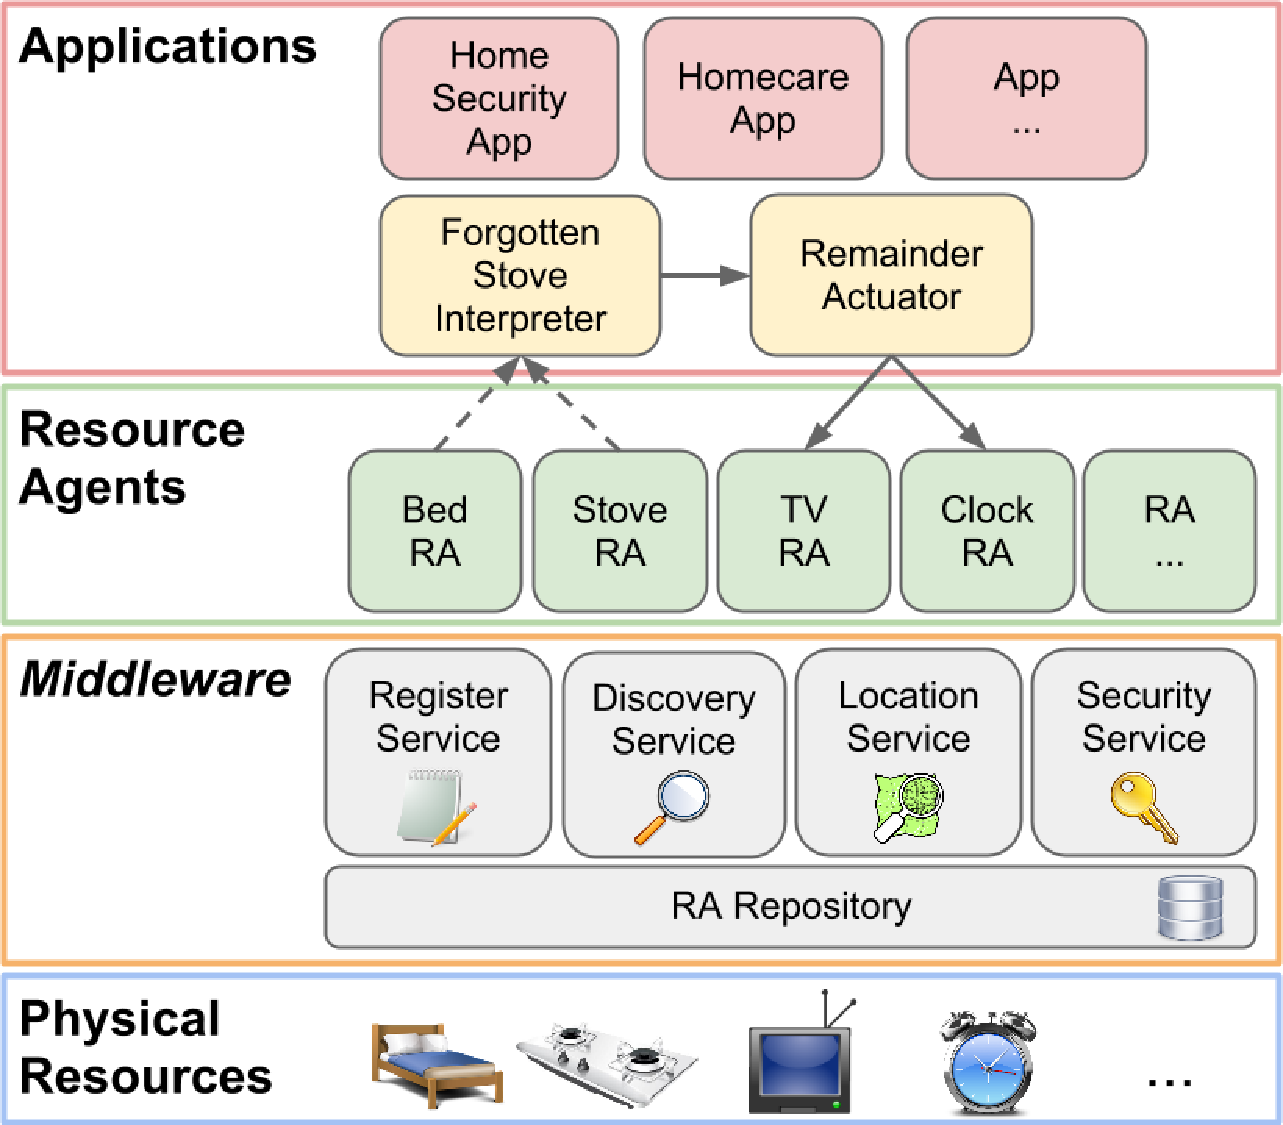
\includegraphics[width=3.5in]{figures/architecture-refactored-v2.pdf}
\caption{Framework Layer Architecture}
\label{fig:arch}
\end{figure}

\subsubsection{Physical Resources Layer}
The deepest layer is the one where is found the resources present in the environment. In a IE these resources are the smarter versions of daily used objects, such as beds, stoves, TVs, clocks, and so on. Since all these resources have their own mechanisms of communication and operation, then a higher level entity is required to deal with them.

\subsubsection{Middleware Layer}
This layer comprehends the main services that sustain the interoperability of the RAs and provides basic features to the development of UbiApps. The management services and the RA Repository, that compose the middleware, will be further discussed in Subsection~\ref{subsec:sgar}.
% Below the management services a RA Repository keeps , that  as will be further discussed in Subsection~\ref{subsec:sgar}, 

\subsubsection{Resource Agents Layer}
This layer is composed by all the RAs that represent physical resources already coupled with the IE. The RA will be presented in Subsection~\ref{subsec:ra}.

\subsubsection{Applications Layer}
The higher layer includes all UbiApps that are enjoying the middleware features and also all the software level RAs, which are represented in the figure by the ``Forgotten Stove Interpreter'' and the ``Remainder Actuator''.


% %%%%%%%%%%%%%%%%%%%%%%%%%%%%%%%%%%%%
%              SECTION
% %%%%%%%%%%%%%%%%%%%%%%%%%%%%%%%%%%%%
\section{Framework Features and Application}This section approaches the main features provided by the framework, which includes the definition of the RA (Subsection~\ref{subsec:ra}), the management services (Subsection~\ref{subsec:sgar}) and the context interpretation (Subsection~\ref{subsec:ci}). In the next section we will present the current status of the implementation.
% This section approaches the main features provided by the framework, which includes the definition of the RA (Subsection~\ref{subsec:ra}), the management services (Subsection~\ref{subsec:sgar}) and the context interpretation (Subsection~\ref{subsec:ci}). Also, based on the reference implementation, an application was built to provide a tool for the prototyping, management and visualization of applications and resources running on the IE.

  \subsection{Resource Agents} \label{subsec:ra}
  % [resource]
  % A resource may be defined as any hardware or software entity that exposes services which can be used by other entities and applications present in IE. Thus, sensors, actuators and smart devices (e.g. stove, fridge, air-conditioning) fall within this definition. For example, a light bulb can expose a service to get its current state (either on or off) and another to effectively turn it on and off. A software module that monitors all these light bulbs turned on, deduce the power consumption and expose this information is also an example of resource.

  A resource may be defined as any hardware or software entity that exposes services (of data acquisition or actuation) which can be used by other entities and applications present in IE. Thus, sensors, actuators and smart devices (e.g. stove, fridge, air-conditioning), as well as software modules that provide a service to the environment, fall within this definition. 

  The RAs are entities that represent resources. They encapsulate the specificities of resources and expose their information to the environment through standard interfaces, so that others can access them uniformly reducing the complexity of integration. 

  The Dey and Abowd's definition to context proposes three entities as the most basic of a ubiquitous system, i.e. person, place and object (or thing). Although the difference of concepts, we have conceived all these three entities as RAs on the framework, but observed their particular features. Thus they inherit the convenience of being a RA.

  % The Resource Agents (RA) can be understood as entities that represent resources, which are sensors, actuators, devices, and smart appliances, as well as software modules that provide a service to the environment. The RAs encapsulate the specificities of resources and expose their information to the environment through standard interfaces, so that others can access them uniformly reducing the complexity of integration. For example, data collection details from a temperature sensor would be known only by their RA, which is responsible for providing a simple interface to other system components.
  %it's similar to the widget of the context toolkit
  %enjoys benefits of SOA

  %From gator tech:
  %decoupling sensors and actuators from sensor platforms ensures openness and makes it possible to introduce new technology as it becomes available

  [wrapper]

    \subsubsection{RA Interfaces}

    The RA architecture includes two interfaces for input and output. The former is called Context Variable (CV) and is responsible for exposing the RA's context information. The latter is called Operation (OP) and is responsible for exposing features (or actuation services) belonging to RAs, enabling applications to actively interact in the environment.
    % In the previous example, the ``oven is turned on'' and the ``oven temperature in �C'' are the some of the RA's CVs. 

    Consider the simple example of a smart stove where the instantiation of its RA exposes services to get its current context (e.g., oven is turned on, oven temperature in $\,^{\circ}\mathrm{C}$) and services that may change its context (e.g., turn oven off, set temperature as $150\,^{\circ}\mathrm{C}$). Hence, the RA concept meets the first challenge (i), which is the \textit{devices heterogeneity}, since decoupling sensor and actuator from the sensor platforms favors the flexibility. %FIXME: is it right?

    % The RA are distributed components that can be used to 


    \subsubsection{Communication}

    % [communication mechanisms]
    % The communication performed between two different ARs or between an AR and an application is developed through '
    % Towards implementing 
    In order to meet requirements typical of distributed environments, two communications mechanisms have been included in the framework: the Remote Procedure Call (RPC), that implements synchronous communication; and a publish-subscribe mechanism (pub-sub)~\cite{eugster2003many}, that implements asynchronous communication. The RPC is used to access directly the RA, querying for its context by accessing its CVs, or calling its OPs. On the other hand, through the pub-sub a RA can subscribe to a CV of another one (consumer) and further receive a notification, when the first RA publishes its CV state change (provider).

    The RA has a domain name, the RA Name System (RANS), that allows its unique identification in the IE. This identification is similar to the DNS, where the name remains the same even if the network address (IP) changes, the only change is the updating of the addressing table. 

    \subsubsection{RA Structure}
    In analogy to object-oriented programming we define classes of RAs to represent the type of the resource with specific interfaces. Besides other informations present in the AR's structure (such as name, location, subscribed RAs, among others) it has its type hierarchy. The type hierarchy is composed by a sequence of classes that classify the entity and has been inspired by the ontology described by Ranganathan~\cite{ranganathan2005olympus}. In the Subsection~\ref{subsec:sgar} we will present how this feature can be used to find a RA and to define its functionalities.


  \subsection{Resource Management Support Service} \label{subsec:sgar}
  A set of services is responsible for providing basic functionalities to manage the RAs. The four main services are the RA Register Service (RRS), the RA Discovery Service (RDS), the RA Location service (RLS) and the Security Management Service (SecMS). All these services access the RA Repository (RR) that maintains informations about the RAs (addresses and descriptions) and the map data structure (map of the environment). The Figure~\ref{fig:arch} represents, in the Middleware layer, the RR and above it the management services.

  The management services are also designed as RAs, hence they take advantage of the communication mechanisms already provided by it and communicate using the same primitives. 

    \subsubsection{RA Register Service} 
    The RRS allows the registration and deregistration of RAs instances references and description. This service also has CVs that allows the developer to know when RAs enter and leave the IE

    The naming and addressing scheme can be generalized to work over the internet, and comply with the internet of things concept.

    \subsubsection{RA Discovery Service}
    The RDS allows the search for registered RAs based on specific attributes, which are the RA name, RANS and type. The search by RANS will only return one RA, but the search by name or type will return all RAs that meet this criteria.

    After the discovery of a RA, the stakeholder can instantiate a stub (i.e. a proxy) of this RA, when both the stub and the current implementation of the RA implement the same interface. Through the stub the CVs and OPs can be accessed, what internally will be converted to network calls to the RA object (RPC functioning). 

    During the application initialization the only information required get started is the RDS address. And even this information can be obtained, if within a LAN, by sending a broadcast message with the request; or using the DNS, if within a WAN. With the RDS address on hands any RA can be found, including the other management services (i.e., the RRS, RLS and RSS). 
    %, before doing the connections to RAs,

    \subsubsection{RA Location Service}
    The RLS explores the map of the environment to run the required queries. This service performs searches related to the location of RAs, such as the physical location of RAs, the RAs located on some place, the RAs of some type located on some place, the RAs close to another and order by proximity, among others. Thus, if a developer needs audiovisual devices close to some person, for example, she can run this search through the RLS and will receive a list, where an utility function can choose the more relevant result.

    The RLS exposes CVs that allows not only the query for if a RA is located at some place, but also to subscribe to that place for the sake of being notified of the entrance or exit of a specified RA type. Therefore, even if the RA is still not registered, an application can subscribe to a place and wait for its appearance.

    Nowadays there are several technologies to map and/or track the location of entities, that may include from people to small things. These technologies vary mainly based on precision, ubiquity (capable of being ``invisible'') and price. As examples we have the GPS, the smart floor, cameras (associated to image processing softwares), Wi-Fi triangulation, RFID tags, and so on. In this approach we do not comply with any specific technology, and we assume that the RA can discover its own location or the RLS can.
    % already established technology of location

    \subsubsection{Security Management Service}
    The security concern is always a central topic on UbiComp systems, moreover because of diverse aspects of security required. Some aspects are already inherited depending on the technology adopted, e.t., the Wi-Fi already ensures against the registration of outside devices and the exchange of informations.

    [credentials]

    [domains]
    % The SecMS manages both the user's credentials and the application's domains.
    % 
    % On the 

  \subsection{Context Interpretation} \label{subsec:ci}
  % [directly programmed]
  The context interpretation serves to aggregate context information from different sources in accordance with some specific logic and considering the passage of time. This logic is defined by the developer and the interpretation is implemented with the framework's support. %The CI concept was inspired by the Aggregator in Dey and Abowd~\cite{dey2001conceptual} whose objective was to gather logically related context and provides them in a single component.
  
  The entity that performs the context interpretation may be encapsulated by a RA, thus allowing the subscription to other RAs, what is called Context Interpreter (CI). This concept allows dealing with context in a higher level and also provides a separation on concerns, since a context interpreter decouples the steps for context acquisition, evaluation, timing and notification, that are repeatedly performed by the UbiApps. Therefore, using the CIs also promotes the reuse, either by the creator application or by other ones. 
  %FIXME: Doubt: ``a RA'' or ``an RA''?
  
  The framework uses a generic approach for creating context rules, which are composed by two parts: the interpretation and the actuation. The interpretation part, as already stated before, concerns on binding the CI itself with CVs from different RAs, evaluating the expression that interrelates those CVs, and notifying whoever is interested. The actuation part is a RA that is subscribed to the CI, and develop some job, that may change the context of the IE or change some state in a software level.
%   in which developers are able to define the logic of the rule in the application using the framework support for context acquisition, as well as to perform actions on the environment. 
  
  The Figure~\ref{fig:arch} shows on Applications Layer an examplo of a context rule with two components: the CI (``Forgotten Stove Interpreter'') and the actuator (``Remainder Actuator''). In this simple example, the CI is subscribed to the RAs ``Bed RA'' and ``Stove RA'', and internally it contains the following rule expression: ``bed is occupied and stove is on for T min''. The actuator, awaits for when the condition of the CI met for triggering its action that, in case, is to play the clock's alarm sound and to show on TV a message saying that ``the stove has been forgotten''.
  
%   A avalia��o da express�o � desempenhada pelo pr�prio IC quando o contexto muda. A atua��o ocorre quando um agente atuador � subscrito � um IC, recebendo assim a notifica��o de que a express�o da regra foi avaliada como verdadeira. Estes agentes atuadores podem tanto ser atuadores simples, que desempenham a��es sequencialmente no ambiente utilizando OPs diretamente (e.g., desligar l�mpada, gravar programa��o de determinado canal da TV); como atuadores mais complexos, que executam a��es n�o necessariamente baseadas em OPs (e.g., execu��o de algum outro software, que utiliza um canal de emerg�ncia do servi�o de sa�de ou bombeiros).

  [talk more about actuators]
  
  [can have many actuators]

  [timer can be CV]
  
  [how to aggregate others standards such as rule engines]
%   Thus, developers can use their own standards, if appropriate. An alternative approach implemented in the context of middleware is to use the Context Processors (see Section 3.2).
  
%   The CI concept was inspired by the Aggregator in Dey and Abowd~\cite{dey2001conceptual} whose objective was to gather logically related context and provides them in a single component. However, in our approach, the information gathered compose a context rule whose evaluation returns true or false, and triggers an actuator listener. 
  
  
  
  Through the CI the framework address the challenge (ii), which is related to the amount and diversity of context informations and services, since the context interpretation allows the autonomous behaviour of RAs.
  
%   The RA can be used to aggregate informations come from other RAs similarly to the Aggregator presented by Dey and Abowd~\cite{dey2001conceptual}.

  
%. This concept allows dealing with context in a higher level so that developers are free to focus on their business logic
  
\section{SmartAndroid}
[android and other techs]

[we have implemented most of the framework features, thought much more remain to be done]

  \subsection{Distributed Components Model}
  [implementation of RA and services]

  \subsection{Context Rules Parsing}
  [implementation of context rules]
  %   Support the interpretation of the context framework enables a separation of concerns, where developers abstract implementation of contextual rules and focus on the application logic.
  
  \subsection{Context Rules Running}
  
  [context rules conflicts is an ongoing study that aims at discover a conflict in runtime,]
  
  \subsection{Interface for Management and Prototyping} \label{subsec:ipgap}
  % interface de prototipagem e gerenciamento de aplica��es pervasivas
  % prototyping and management of pervasive applications interface
  % pervasive applications' management and prototyping interface
  % PAMPI
  % management and prototyping interface MPI
  [description]

  [main figure]

  [rules composer]



% %%%%%%%%%%%%%%%%%%%%%%%%%%%%%%%%%%%%
%              SECTION
% %%%%%%%%%%%%%%%%%%%%%%%%%%%%%%%%%%%%
\section{Application Examples} \label{sec:evaluation}



% %%%%%%%%%%%%%%%%%%%%%%%%%%%%%%%%%%%%
%              SECTION
% %%%%%%%%%%%%%%%%%%%%%%%%%%%%%%%%%%%%
\section{Conclusion} \label{sec:conclusion}
The conclusion goes here.


% %%%%%%%%%%%%%%%%%%%%%%%%%%%%%%%%%%%%
%              SECTION
% %%%%%%%%%%%%%%%%%%%%%%%%%%%%%%%%%%%%
% use section* for acknowledgement
\section*{Acknowledgment}
The authors would like to thank CNPq and FAPERJ for partial funding of this work.


% references section
\bibliographystyle{IEEEtran}
\bibliography{references}




% that's all folks
\end{document}
